\section{DS2}
\textbf{Die Biodiversitätskarten zeigen:} Taxonomische Diversität (Artenreichtum) pro Region steigt an:
\begin{itemize}
	\item Von den Polen zum Äquator
	\item Von Gegenden mit ungünstigen Wachstumsbedingungen (zu kalt, zu trocken) hin zu Gegenden mit günstigeren Bedingungen (konstant warm und feucht)
\end{itemize}

\subsection{Breitengradient}
\begin{itemize}
	\item Es existiert eine starke Korrelation zwischen geographischer Breite und Artenvielfalt (hier Pflanzenarten) – vor allem dort, wo die Klimagradienten besonders stark ausgeprägt sind (siehe Mutke \& Barthlott (2005))
	\item Breitengradienten existieren nicht nur bei Pflanzen (z.B. Termiten, Vögel, Säugetiere)
	\item Ausnahmen: Gymnospermen, parasitoide Hymenoptera, 
\end{itemize}

\textbf{Was verbirgt sich hinter der Breite?} Viele Faktoren variieren mit der Breite:
\begin{itemize}
	\item Mittlere Temperatur $\downarrow$ (Die mittlere Jahresmitteltemperatur folgt der Einstrahlungsintensität, d.h. Nordpol $\downarrow$ Äquator $\uparrow$ Südpol $\downarrow$)
	\item Mittlere Niederschlag $\downarrow$
	\item Variabilität (T, NS) $\uparrow$
	\item Netto-Primärproduktion\footnote{Produktion organischer Substanz durch Photosynthese oder Chemosynthese, abzüglich des Verlustes durch Gesamt-Atmung (Tages- und Nachtatmung aller grünen und nicht-grünen Pflanzenteile) \\ \url{http://www.spektrum.de/lexikon/biologie/nettoprimaerproduktion/46072}} $\downarrow$
	\item Glazialgeschichte, Evol. Zeit $\downarrow$
	\item Fläche ($\downarrow \uparrow$)
\end{itemize}

\newpage
\subsection{Übersicht der Erklärungsmuster}
\begin{itemize}
	\item \textbf{Art-Areal-Beziehung}
	\item \textbf{Energie-basierte Hypothesen}
	\begin{itemize}
		\item Mehr-Individuen-Hypothese (u.a. Hutchinson 1959, Srivastava 1998)
		\item Metabolische Theorie der Diversität (Allen et al. 2002)
	\end{itemize}
	\item \textbf{Evolutionsbasierte Hypothesen}
	\begin{itemize}
		\item Zeitbasierte Hypothesen (incl. Nischenkonservativismus, Toleranzhypothese)
		\item Speziationshypothese
		\item Extinktionshypothesen
	\end{itemize}
\end{itemize}

\subsubsection{Art-Areal-Beziehung}
\begin{itemize}
	\item Generelles Prinzip in der Ökologie
	\item $S=c \cdot A^z$ mit S: Artenzahl, A: Fläche, z, c: Parameter, z (Exponent/ Steigung) $\approx$ 0.25 – 0.30
	\item logarithmische Kurve: 50\% Habitatverlust $\sim$ 10\% Artenverlust, 90\% Habitatverlust $\sim$ 50\% Artenverlust, 99\% Habitatverlust $\sim$ 75\% Artenverlust (Artenreichtum über Fläche)
\end{itemize}

\textbf{Mechanismen}
\begin{itemize}
	\item Artefakt?: Auf größeren Flächen können insgesamt mehr Individuen gesammelt werden als auf kleinen. Daher ist die Wahrscheinlichkeit größer, mehr Arten zu finden.
	\item Habitatdiversität: Größere Flächen sind topographisch/edaphisch diverser $\rightarrow$ mehr Habitate $\rightarrow$ mehr Möglichkeiten für unterschiedliche Arten zu existieren
	\item Artbildung/Extinktionsdynamik: größere Fläche $\rightarrow$ größeres potentielles Areal von Arten $\rightarrow$ größere Wahrscheinlichkeit der Artbildung (mehr Barrieren) und kleinere Wahrscheinlichkeit des Aussterbens (mehr Individuen)
\end{itemize}

\textbf{Fazit: Art-Areal und Diversitätsgradient}
\begin{itemize}
	\item Rezente Verteilung der Landmassen nicht kompatibel mit den globalen Mustern
	\item Logarithmischer Zusammenhang könnte selbst bei entsprechender Landverteilung den starken Anstieg zu den Tropen nicht erklären
\end{itemize}

\subsubsection{Mehr-Individuen-Hypothese}
\begin{itemize}
	\item Produktivität (NPP = Netto-Primärproduktion) limitiert die Anzahl der Individuen
	\item In tropischen Gebieten ist es wärmer und feuchter, NPP ist höher in den Tropen, es ist Platz für mehr Individuen
	\item Wenn die Populationsgrößen nicht mit NPP variieren, dann ist Platz für mehr Arten!
\end{itemize}

\begin{itemize}
	\item Mehr Energie, höhere NPP
	\item Es gibt einen positiven Zusammenhang zwischen NPP und Individuendichte
	\item Es gibt einen positiven Zusammenhang zwischen Individuendichte und Artenreichtum
\end{itemize}

\textbf{Zusammenhang:}\\
\begin{tabularx}{\textwidth}{p{0.45\textwidth}p{0.55\textwidth}}
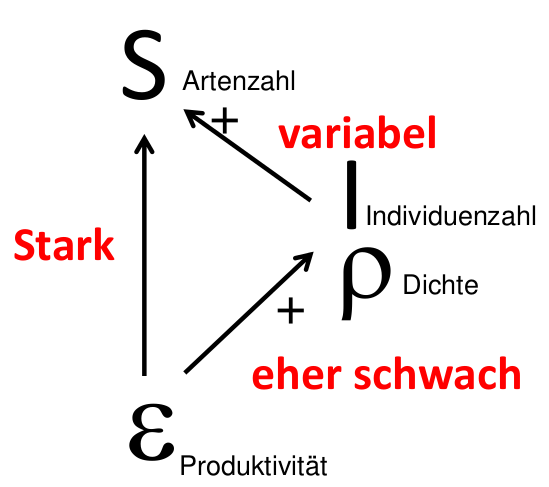
\includegraphics[width=0.45\textwidth]{lectures/DS2/pix/pic1.png} &
Sollte der Pfad über die Dichte/Individuenzahl den Mechanismus erklären, so müssten die „proximaten“ Zusammenhänge (also $\varepsilon$ vs. $\rho$/I und $\rho$/I vs. S) stärker sein als der distale ($\varepsilon$ vs. S) \textbf{Dies ist nicht der Fall!}
\end{tabularx}
\\\\
\textbf{Fazit: Mehr-Individuen-Hypothese}\\
Angesichts der Datenlage eher nicht wahrscheinlich
\begin{itemize}
	\item Verbindung zwischen Energie und Dichte/Individuenanzahl eher schwach
	\item Änderungen der Dichte mit der Breite nicht in der richtigen Größenordnung (zu schnell)
\end{itemize}

\newpage
\subsubsection{Metabolische Theorie der Diversität}
\begin{itemize}
	\item Körpertemperatur = Umgebungstemperatur
	\item Wärmer $\rightarrow$ mehr metabolische Energie pro Individuum
	\item Annahme, dass Energienutzung durch Population konstant: wärmer $\rightarrow$ kleinere Populationen und/oder kleinere Individuen
	\item Individuenzahl pro Gemeinschaft variiert nicht geographisch $\rightarrow$ höhere Diversität
\end{itemize}

\textbf{Fazit: Metabolische Theorie der Diversität}\\
\textcolor{red}{passt auch nicht... warum???}

\newpage
\subsubsection{Evolutionsbasierte Hypothesen}
Sind die Tropen die „Wiege“ oder das „Museum“ der Diversität?

\begin{itemize}
	\item \textbf{Evolutionszeit} (=„Museum“)
	\begin{itemize}
		\item Tropische Regionen sind erdgeschichtlich älter, viele Taxa haben Ursprung in den Tropen
		\item Verbreitung aus den Tropen heraus ist limitiert
	\end{itemize}
	\item \textbf{Diversifizierungraten} (=„Wiege“)
	\begin{itemize}
		\item Genetische Drift in kleineren Populationen hat höhere Artbildungsraten zur Folge (Federov 1966)
		\item Klimavariabilität hat in den Tropen höhere Artbildungsrate zur Folge (Haffer 1969)
		\item Höhere Wahrscheinlichkeit von parapatrischer (Moritz 2000) und sympatrischer Artbildung (Gentry 1989)
		\item Größere Fläche bewirkt größere Wahrscheinlichkeit von Isolation (Terborgh 1973)
		\item Geringere physiologische Toleranzen erschweren die Verbreitung und fördern die Isolation (Janzen 1967)
		\item Höhere Temperaturen bedingen höhere Mutationsraten und damit Artbildungsraten (Rohde 1992)
		\item Stärkere biotische Interaktionen führen zu höherer Spezialisierung und höherer Artbildungsrate (Dobzhansky 1950, Fischer 1960)
	\end{itemize}
	\item \textbf{Extinktionsraten}
	\begin{itemize}
		\item Geringere Klimavariabilität reduziert Extinktionsrisiko (Darwin 1859)
		\item Größere Fläche, höhere Populationsgrößen, reduziertes Extinktionsrisiko (Rosenzweig 1995)
	\end{itemize}
\end{itemize}

\textbf{Das Argument „Zeit“:} die Tropen sind älter und konnten daher eine größere Anzahl von Arten akkumulieren („fair chance“). Die nördlicheren Regionen sind durch Klimavariabilität, v.a. Eiszeiten, stärker in Mitleidenschaft gezogen worden $\rightarrow$ \textbf{jedoch sehr unterschiedlich (Vergleich USA, Europa, Asien)}